\documentclass[a4paper]{article}

\usepackage[]{geometry}
\geometry{
	a4paper,
	left=20mm,
	right=20mm
}
\usepackage{float}
\usepackage[version=4]{mhchem}
\usepackage[english]{babel}
\usepackage[utf8]{inputenc}
\usepackage[T1]{fontenc}
\usepackage{textcomp}
\usepackage{rsc}
\usepackage{amsmath, amssymb}
\usepackage{mathtools}
\usepackage{siunitx}
\usepackage{sectsty}
\subsectionfont{\normalfont\itshape}

\usepackage{caption}
\captionsetup[figure]{font=small}

\edef\restoreparindent{\parindent=\the\parindent\relax}
\usepackage{parskip}
\restoreparindent

\usepackage[]{multicol}

% figure support
\usepackage{import}
\usepackage{xifthen}
\pdfminorversion=7
\usepackage{pdfpages}
\usepackage{transparent}

\graphicspath{{Chapters/}}

\pdfsuppresswarningpagegroup=1
\counterwithin{equation}{section}

\newcolumntype{L}{>{\centering\arraybackslash}m{5cm}}
\newcommand{\wrap}[1]{\parbox{.33\linewidth}{\vspace{1.5mm}#1\vspace{1mm}}}


\title{A comparison of methane decomposition and water splitting reaction methods as a means to produce molecular hydrogen.}
\author{E. Lunnon, A. Nicholson, W. Ogle, N. Simons}

\begin{document}
\maketitle
\tableofcontents
\clearpage

\section*{Abstract}%
\label{sec:abstract}
The widespread use of fossil fuels is a major environmental issue, due to the release of greenhouse gases contributing to global warming.
Therefore, it is necessary to find an alternative, \ce{H2} could be a promising option, however problems persist in current methods for generation of \ce{H2}.
In this review we discuss the current methods of steam methane reformation and uncatalysed water electrolysis for the production of hydrogen and evaluate potential novel methods involving both methane and water as potential feedstocks.

The methane methods evaluated in this review are the thermal decomposition of methane using \ce{Ni} catalyst on a hydroxyapatite support and radical methane pyrolysis.
Radical methane pyrolysis displayed around a \SI{90}{\percent} decrease in enthalpy cost when compared to the traditional steam methane reformation, which is a significant energy saving.
The water electrolysis methods we looked at are solid oxide electrolytic cells and acidic/alkaline amphoteric electrolytic cells.
The latter achieved an energy consumption \SI{30}{\percent} less than conventional alkaline electrolysis.

These new methods have clear improvements over current methods in terms of energy cost, which makes the production of \ce{H2} using renewable energy a viable option.
This would transform the way we store and release energy.



%\clearpage

\begin{multicols}{2}
\section{Introduction}%
\label{sec:introduction}
As the global energy demand continues to increase, a sustainable alternative to fossil fuels is desperately needed.
\ce{H2} potentially presents an innovative solution, but the energy costs for production are currently prohibitive.
An efficient synthesis could be a revolutionary step towards a more sustainable future, as the hydrogen fuel cell has many advantages over current energy sources; a hydrogen storage tank can be refilled much more quickly than a battery can be recharged, \cite{Offer2010} making it far more practical for use in transport.

In a fuel cell, electricity is produced by reducing oxygen at the cathode \eqref{eq:1.1} and hydrogen at the anode \eqref{eq:1.2}.
\begin{align}
	\ce{O2 + 4H+ + 4e- &-> 2H2O}	\label{eq:1.1}\\
	\ce{2H2 &-> 4H+ + 4e-} 		\label{eq:1.2}
\end{align}
This reaction leads to the production of only heat, water and electricity, \cite{6278114} which is a major advantage over systems which produce \ce{CO2}.
These reasons alone make investigating the sustainability of hydrogen production a worthwhile endeavour.

We will start by discussing the traditional methods of synthesis and where they fall short of the criteria required to produce hydrogen sustainably.
\cite{Saxena2011} Then we will look at new approaches in the areas of methane decomposition and water electrolysis reactions.
The two methane methods are methane decomposition using an \ce{Ni} catalyst with a hydroxyapatite support, and radical methane pyrolysis.
The two water electrolysis methods are electrolysis with an acid/alkaline amphoteric cell and solar powered steam electrolysis using a solid oxide electrolytic cell.

We will then compare these new methods with the traditional methods; evaluating these new methods and investigating their sustainability compared with their traditional counterparts.
The most promising method from each feedstock will be analysed further, concluding on if and how these new approaches can solve the problems preventing widespread adoption of hydrogen as a fuel.
We will focus on how these new reactions can improve the rate of reaction, allow for more mild reaction conditions, and reduce the cost of reactions, particularly in terms of energy.

We are concerned with the environmental impact of these processes, however discussing the implications of these at scale is beyond the scope of this review.
The practical problems of scaling up will not be discussed in this review however.
We will also not evaluate the uses of the hydrogen when generated, such as potential issues with and improvements to the hydrogen fuel cell itself.



\section{Traditional Methods}%
\label{sub:Traditional_Methods}
\subsection{Steam methane reformation}%
\label{sub:steam_methane_reformation}

The steam methane reformation reaction is an extremely inexpensive and widespread method for producing molecular hydrogen in a commercial setting.
The reaction follows the scheme\cite{Saxena2011}:
\begin{align}
	\ce{CH4(g) + H2O(l) &-> 3H2(g) + CO(g)} \label{ce:steam-reformation}\\
	\Delta H &= \SI{379}{\kilo\joule},\ \SI{1500}{K} \nonumber
.\end{align}
There is also a secondary mechanism for extracting hydrogen from the carbon monoxide by-product of this first stage reaction, which runs at a lower temperature and is called a water gas shift reaction\cite{Chen2008,Saxena2011}.
\begin{align}
	\ce{CO + H2O &-> CO2 + H2}\label{ce:water-shift} \\
	\Delta H &= \SI{-41.1}{\kilo\joule\per\mole},\ \SI{1200}{K} \nonumber
.\end{align}
This basic reaction scheme is applied to generate approximately 40\% of the global hydrogen demand\cite{SBN2020}; primarily due to using readily available reagents, it is a mature technique and it is inexpensive.

Although both reactions \eqref{ce:steam-reformation} and \eqref{ce:water-shift} can proceed without the use of a catalyst one is often employed for the water gas shift reaction \eqref{ce:water-shift} in order to increase the hydrogen yield.
Iron-chromium or copper-zinc compounds are often used dependant on if the reaction is a low- or high-temperature shift. 

Unfortunately this method doesn't produce hydrogen in a sustainable way; the production rate without the gas shift reaction is low, and produces one equivalent of \ce{CO} for every three of \ce{H2}.
When the gas shift reaction is used this toxic carbon monoxide is used to generate further \ce{H2}, as well as the pollutant gas \ce{CO2}.
Placing additional strain on the planet by up scaling steam reformation processes will only lead to further damage of the planet, so this process is not useful when considering fuelling a hydrogen powered society.


\subsection{Uncatalysed electrolysis of water}%
\label{sub:uncatalysed_electrolysis_of_water}

Water electrolysis is another basic technique for extracting hydrogen, this time from water.
Water is an incredibly naturally abundant chemical making up a large fraction of the earth's surface.
When hydrogen is consumed by a fuel cell, water is the sole by-product.
Water can be split into hydrogen and oxygen via an electrolytic cell, where at the anode reaction \eqref{eq:UC_oxidation} occurs and at the cathode reaction \eqref{eq:UC_reduction} occurs.
\begin{align}
	\ce{2H2O &-> 4e- + 4H+ + O2} \label{eq:UC_oxidation} \\
	\ce{2H+ + 2e- &-> H2} \label{eq:UC_reduction}
.\end{align}
A common choice of electrolyte for these kinds of cells is \ce{KOH}; an alkaline cell is more efficient\cite{merrill2006}.
\ce{KOH} has the highest charge mobility and solubility in water of the group I and II hydroxides, which makes it the best choice in this case.

Catalytic design is important as when uncatalysed, the electrolytic approach to inter converting  \ce{H2}, \ce{O2} and  \ce{H2O} is not feasible.
In acidic or alkaline solution, the standard cell potential for an electrolytic cell splitting water is equal to the standard potential generated from recombination in a fuel cell, \SI{1.23}{\volt}\cite{Peng2020}.
In practice however, there are many barriers to this reaction which result in uncatalysed cells always requiring a potential difference greater than \SI{1.80}{\volt}.
There are various practical issues which cause the greatly decreased efficiency; resistance inside the cell due to work required to move protons, product gasses resulting in a bad connection between the surface of the electrode and the electrolyte, and resistances outside the cell such as the work required for electrons to be conducted through a wire.

Uncatalysed electrolysis is a foundational method on which the water splitting methods is built - catalysts are often deposited on the anode and cathode to lower the reaction barrier and reduce the overpotential that afflicts this method.
There are many possible catalysts, almost all of which involve adsorbtion of protons onto the electrode surface followed by the addition of two supplied electrons, as given in equation \eqref{eq:UC_hads}\cite{Leonard2012}.
\begin{align}
	\ce{H+ + e- &-> H_{ads}}\\
	\ce{2H_{ads} &-> H2}\\
	\ce{H+ + e- + H_{ads} &-> H2} \label{eq:UC_hads}
.\end{align}
Solving the problems with overpotential using safe, effective and cheap catalysts is a promising area of study which could lead to electrolytically generating hydrogen on an industrial scale.

\subsection{Discussion of traditional methods}%
\label{sub:discussion_of_traditional_methods}
Both of these methods discussed offer the potential for large scale hydrogen generation; albeit at a cost.
For MSR the price is paid with high emissions into the atmosphere, with the current \ce{CO2} emissions crisis this isn't a viable way to solve the problem of city-scale energy fixation into \ce{H2}.
For electrolysis, overpotential related to several inferences with the method makes it enviable for similar reasons; the energy to create the \ce{H2} must come from somewhere.
Renewable energy sources currently account for \SI{27}{\percent} of the global energy supply as of 2020\cite{IEA2020} (projected), with much of the rest coming from fossil fuels.

Electrolytic methods currently have fewer environmental problems to solve, but tend to be inefficient which is a major problem when considering the application to energy storage.
There is much research into addressing this inefficiency; modified catalytic electrodes have taken major steps to increase the rate of gas evolution at lower potentials, and entirely different techniques utilising steam at high temperatures address scaling and efficiency concerns.

Methane steam reformation itself is a technique which has been improved in efficiency and yield over the years it has been used; membrane reactors \cite{} modifications to the gas-shift reaction \eqref{ce:water-shift}\cite{Saxena2011} show promise.
Other approaches to using methane as a feedstock are discussed in this review, ones which can take the same material and obtain the same product without the need to collect \ce{CO2} back out of the atmosphere.


\section{\ce{CH4} methods}%
\label{sub:ch4_methods}
\subsection{Methane decomposition using a hydroxyapatite supported nickel catalyst.}%
\label{sub:methane_decomposition_using_a_hydroxyapatite_supported_nickel_catalyst_}
One method of methane decomposition currently relies on a nickel catalyst, supported by compounds such as \ce{TiO2}, \ce{MgO}, \ce{ZrO2}, \ce{Al2O3}.
The rate of reaction depends on the \ce{Ni} particle size, with both relation to the dispersion and stabilisation by a suitable support\cite{Ashok}.
 J. Ashok, S Naveen. Kumar, M. Subrahmanyam, A. Venugopal, have been looking at how a new nickel catalyst support, hydroxyapatite (\ce{HAp}), and how it will affect this reaction.

 \ce{HAp} is produced from \ce{Ca5(NO3)4.4H2O} and \ce{(NH4)(PO3OH)} to make \ce{[Ca5(PO4)3(OH)]} while under basic conditions\cite{Ashok}.
Unlike the previously mentioned catalyst supports, \ce{HAp} is irreducible; this means no \ce{CO} is made in the reaction unlike the other supports currently in use.
This means the reaction has a simple overall equation with no greenhouse gas (GHGs) emissions:

\begin{align}
	\ce{CH4 -> C +2H2}
.\end{align}

This reaction has an enthalpy of \SI{75.6}{\kilo\joule\per\mole} meaning it is endothermic.
In the experiment performed by J. Ashok et al. the experiment was run at just \SI{650}{\celsius}\cite{Ashok}, as this is an endothermic reaction these operating condition are mild.
The \ce{CH4} should be flowed through the reaction chamber at a slow \SI{24}{\liter\per\hour}\cite{Ashok} again meaning no extra energy is needed to accelerate the gas.
These combined factors and the lack of (GHGs) produced make this reaction both green and sustainable.

\begin{figure}[H]
	\centering
	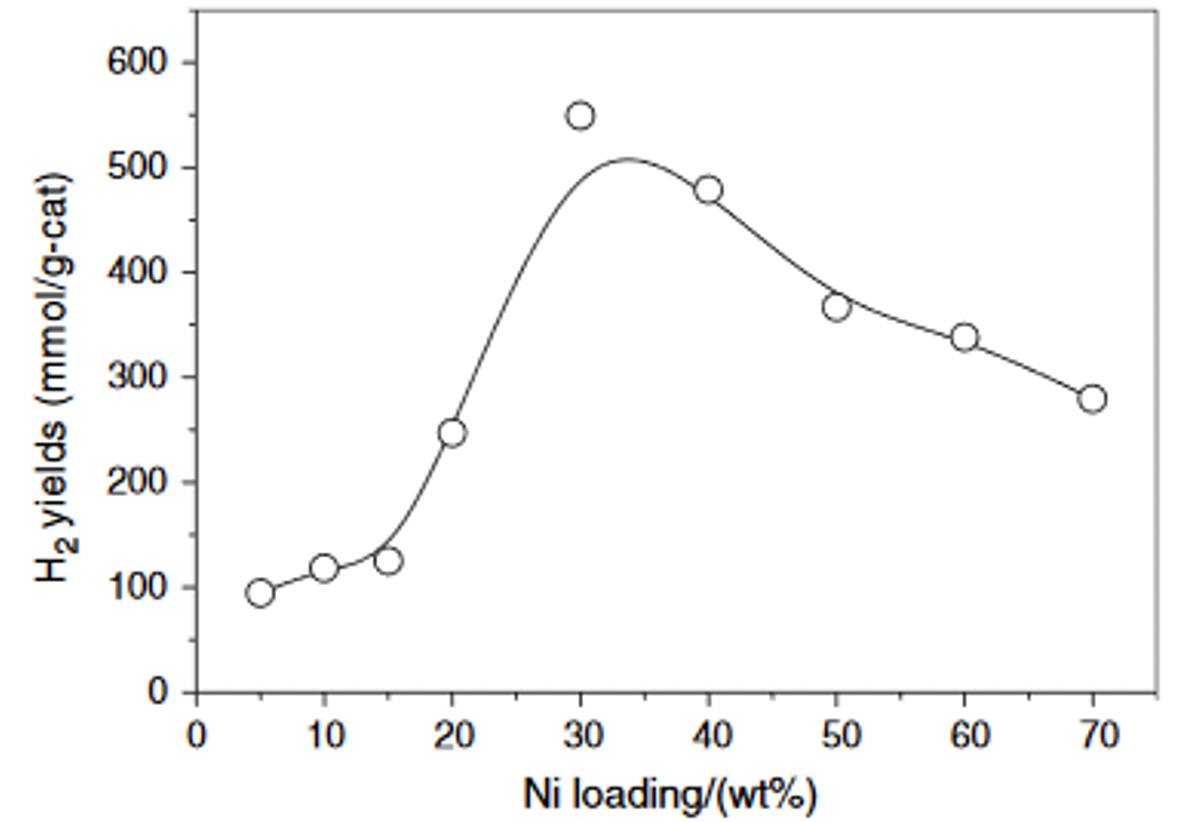
\includegraphics[width=0.4\textwidth]{539a7840-2cb8-11eb-895f-8c8590753a48.png}
	\caption{A plot of percent weight of nickel loaded onto the catalyst support vs \ce{H2} yield.}  
	\label{fig:MD_plot1}
\end{figure}

\begin{figure}[H]
	\centering
	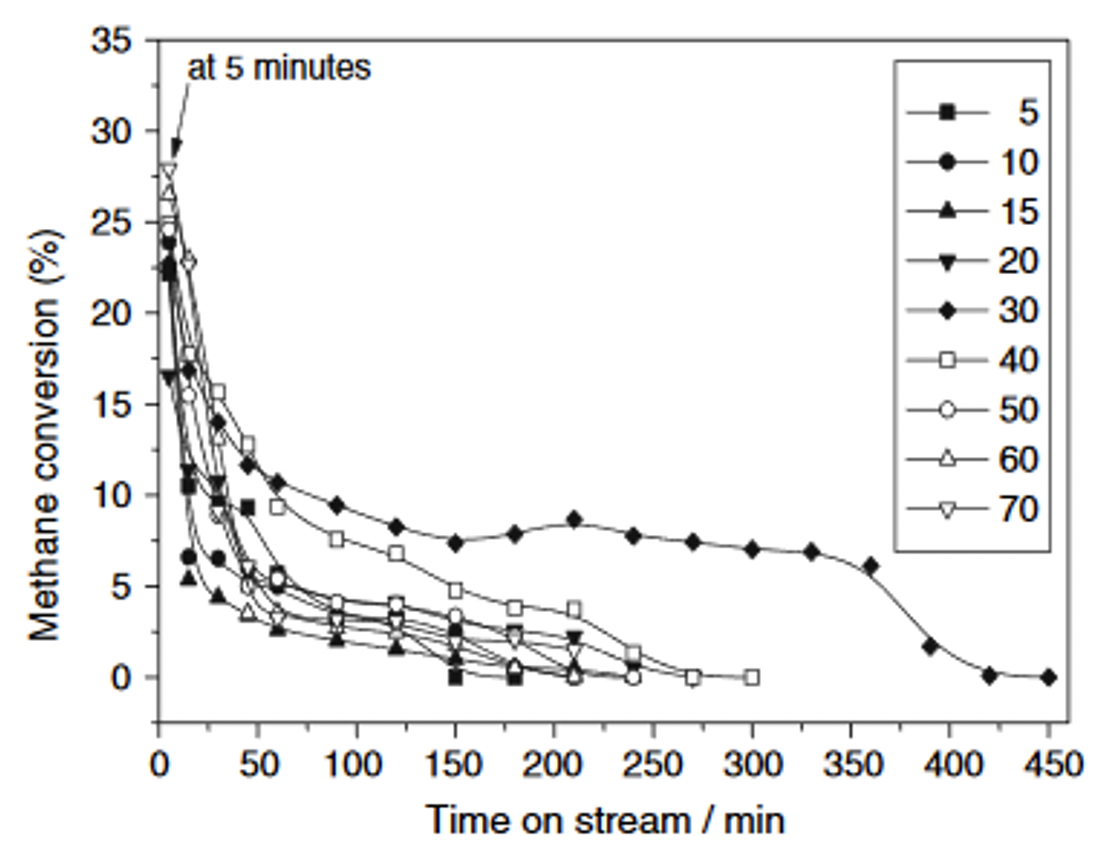
\includegraphics[width=0.4\textwidth]{0ed19cac-2cb8-11eb-895f-8c8590753a48.png}
	\caption{A multiple plot of varying percent weights of nickel loaded onto the support showing how methane conversion efficiency varies with time.}
	\label{fig:MD_plot2}
\end{figure}

As you can see from figures \ref{fig:MD_plot1} and \ref{fig:MD_plot2} a 30 wt\% \ce{Ni} sample was the optimum for this reaction.
It has both the highest yield and the best durability.
This reaction does have one major drawback however in that the catalyst does readily degrade.
This means the solid waste carbon, which is responsible for the deactivation of the catalyst, will be contaminated with toxic \ce{Ni} atoms.
This is a very promising technology which warrants further research, as it can help to solve the current \ce{H2} crisis.


\subsection{Radical chain reactions}%
\label{sub:radical_chain_reactions}
Radical methane pyrolysis is a way of breaking a \ce{CH4} molecule into \ce{H2} and pure carbon.
The initial step is the chemisorption of \ce{CH4}, onto the surface of the catalyst.

\begin{align}
	\intertext{The initiation and rate determining step of the radical break down is:}
	\ce{CH4&-> ^.CH3 + H^.}
	\intertext{Then a series of propagation steps take place with the general equation:}
	\ce{^.CH_{n}&-> ^.CH_{n-1} + H^.}
	\intertext{Until a termination step is reached:}
	\ce{4H^.&-> 2H2}
	\intertext{This gives the overall equation of:}
	\ce{CH4&-> C + 2H2}
.\end{align}

This reaction mechanism gives rise to no waste gases such as \ce{CO2} but does has the issue of elemental carbon production which can lead to the degradation of the catalyst as carbon is deposited upon the catalyst surface.
The reaction conditions for this mechanism follow Le Chatelier’s principals.
The reaction is endothermic with an enthalpy of reaction ($\Delta_{r}H$) of \SI{+37.5}{\kilo\joule\per\mole} which is very low when compared to electrolysis which has an $\Delta_{r}H$ of \SI{+286}{\kilo\joule\per\mole}\cite{sbn2020}.
Due to the endothermic nature of the reaction a high temperature is needed; as there are more moles on the RHS, low pressure is needed.
This is very expensive to maintain.
The methane should also move at a low velocity as increases the contact efficiency between the methane and the catalyst, this results in a higher quantity of methane being adsorbed on the active site of the catalyst which means the catalyst will deteriorate slower.

Various catalysts can be used from metals, molten salts/ metals, or carbon-based catalysts.
The main catalysts in a metal catalysed reaction are nickel and iron, these are particularly useful as a partially filled 3d orbitals accept electrons density from the \ce{CH} bonds destabilising their bond strength as ultimately leading to the breaking of the bond.
These metals allow carbon diffusion through the crystalline structure.
Table \ref{tab:catalystTable} shows a few key aspects of the catalysts and how they affect the operating conditions and overall reaction process.

\end{multicols}
\begin{table}[t]
	\centering
	\caption{Catalytic efficacies, all relative values are compared to nickel.}
	\label{tab:catalystTable}
	%\resizebox{\columnwidth}{!}
\end{table}
\begin{multicols}{2}

\ce{Ni} while an effective catalyst, has a major drawback compared to the other catalyst available: its toxicity results in the waste carbon being contaminated with waste \ce{Ni} catalyst.
 
\ce{Fe} catalytic activity is lower than that of \ce{Ni} however it is more resistant to catalytic deactivation.
This is because carbon has higher rate of diffusion in \ce{Fe}, meaning it does not deposit itself upon the active site of the catalyst.
It also has the advantage of being able to operate at high temperatures \SIrange{700}{1000}{\celsius}.
It is cheaper and less toxic than \ce{Ni}.
\ce{Fe} compounds such as: \ce{[Fe(CO)5]}, \ce{[Fe(cp)2]} have been tested as catalysts.
However, these type of clusters can result in unwanted gases, meaning the \ce{H2} has to be separated from the gaseous mixture decreasing the reaction efficiency.
A catalyst was strong support increases the carbon dispersion and reducibility of the metal along with preventing sintering of metal particles.
However, an excessively strong support may hamper the reducibility of metal oxides.
A supported catalyst has a better performance as it balances the carbon dispersion resulting in a longer lasting catalyst while maintaining the reducibility of the metal species.
There are three types of carbon catalyst highly ordered, less ordered, and disordered.
Disordered carbon catalysts have three valence sites or no coordination sites these are known as high energy sites (HES).
The more HES’s there are the faster the rate as these are thought to initiate the mechanism.
More oxygenated catalysts have a higher activity but release \ce{COx}, this is because as \ce{COx} is produced new active sites are created on the surface of the catalyst.
RMD is a very promising new piece of technology that combines both new and old science.
I believe that RMD with an \ce{Fe} catalyst will go a long way to solve the \ce{H2} problem.

\subsection{Discussion of methane methods}%
\label{sub:discussion_of_methane_methods}
Currently SMR provides around \SI{48}{\percent} of the worlds \ce{H2}\cite{sbn2020}, but this could soon change.
With the development of new reactions and catalyst, new and sustainable methods of \ce{H2} production from methane are on the rise.

\begin{figure}[H]
	\centering
	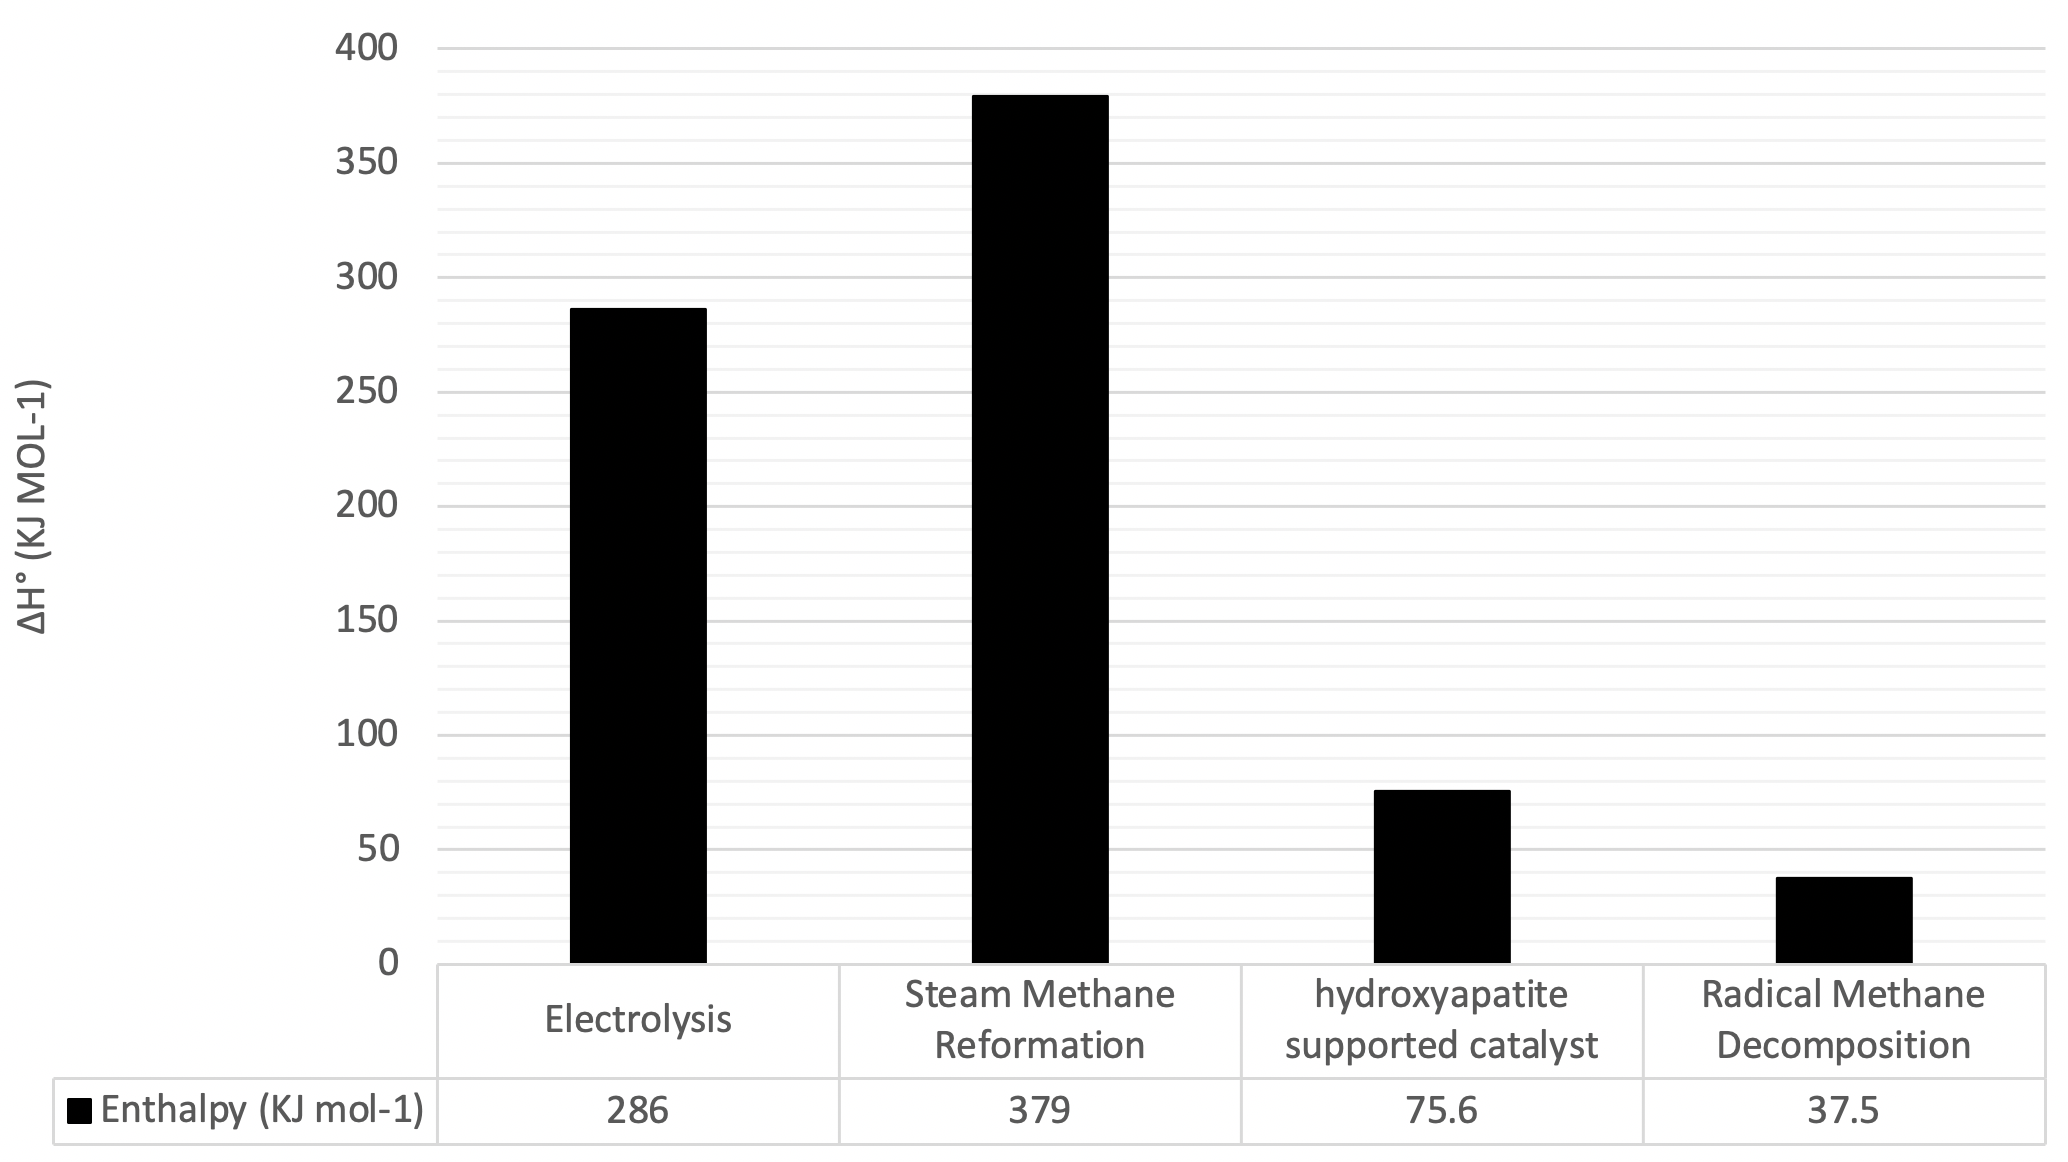
\includegraphics[width=0.4\textwidth]{6b76c760-2cb9-11eb-895f-8c8590753a48.png}
	\caption{A plot showing the enthalpy of the three methane methods alongside uncatalyzed electrolysis as a reference.\cite{SBN2020,Ashok,Saxena2011}}
	\label{fig:ME_disc}
\end{figure}

As you can see from \ref{fig:ME_disc}, radical methane decomposition and hydroxyapatite supported \ce{Ni} catalysts have a significantly lower enthalpy cost meaning they are far more economical processes.

Both \ce{HAp} and RMD both run at much lower operating conditions compared to SMR, this is beneficial not only to the cost of the reaction, but also to the greenness and sustainability.
Further aiding their sustainability is the lack of greenhouse gases produced by both new reactions.
As there are no GHGs produced in either method, no separation step is required to extract the \ce{H2} gas, another positive when compared to SMR.

There are however drawbacks to the new methods of production.
The product is not re-sellable for three reasons: there is not a market for it, the carbon rapidly degrades the catalysts and where \ce{Ni} catalysts have been used, the carbon is contaminated with toxic metal.

Therefore, I believe RMD to be a better method than \ce{HAp}.
RMD has the option of using carbon or molten catalysts whereas \ce{HAp} only uses toxic \ce{Ni} catalysts.
The carbon catalysts have a longer life than metals and also run at lower temperatures.



\section{\ce{H2O} methods}%
\label{sub:h2o_methods}
\subsection{Amphoteric cell}%
\label{sub:some_kind_of_splitting_method_}

An existing H2O electrolysis method which uses an electrolytic cell under alkaline conditions \cite{Zeng2010}, is adapted by adding a membrane and an acidic electrolyte \cite{Lei2019}.

\begin{figure}[H]
	\centering
	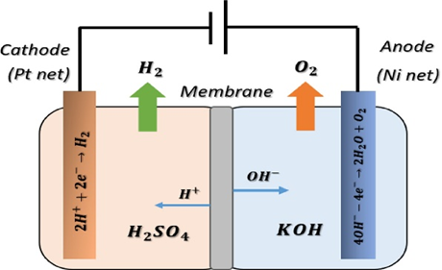
\includegraphics[width=0.4\textwidth]{amphoteric_cell.png}
	\caption{Fig}{Acidic/Alkaline amphoteric electrolytic cell\cite{Lei2019}.}
	\label{fig:amphoteric_cell_diagram}
\end{figure}

An ion-exchange membrane is placed between a \ce{Pt} cathode and an \ce{Ni} anode, this restrains neutralisation between the acidic and alkaline electrolytes.
The \ce{H2SO4} electrolyte provides excess \ce{H+} to react on the surface of the cathode, while the \ce{KOH} electrolyte provides excess \ce{OH-} to react on the surface of the anode.

\begin{align}
	\intertext{\ce{H2} evolution in acidic solution\cite{Lei2019}:} 
	\ce{H3O+ + e- &-> H+ + H2O}\\
	\ce{H3O+ + e- + H^* &-> H2 + H2O}\\
	\intertext{\ce{O2} evolution in alkaline solution\cite{Lei2019}:}
	\ce{OH- &-> OH^* + e-}\\
	\ce{OH- + OH^* &-> O^* + H2O + e-}\\
	\ce{O^* + O^* &-> O2}
\end{align}
(\ce{^*}) - Chemically attaches onto the catalyst.

\ce{H2O} continuously dissociates, the electric potential drives the \ce{H+} into the cathode chamber, and the \ce{OH-} into the anode chamber.
Therefore, the concentration of \ce{H+} and \ce{OH-} in the respective electrolytes is kept high, encouraging the production of \ce{H2} and \ce{O2}.
This results in a lower potential difference for the electrolysis of \ce{H2O}.
Since the experiment took place at a constant current and over a set time, this means that energy consumption was also lower.

So, by using an ion-exchange membrane to separate acidic and alkaline electrolytes, the energy consumption required for the electrolysis of \ce{H2O} was \SI{30}{\percent} less compared to conventional alkaline electrolysis.
If this magnitude of energy efficiency could be achieved on an industrial scale using renewable energy, it would provide a method of producing \ce{H2} from \ce{H2O} without the use of fossil fuels and potentially transform the way we store and release energy.

There is also scope for increased energy efficiency, as increasing temperature led to a lower potential difference for a given \ce{H2} production rate.
This means further research could be undertaken to find the most energy efficient compromise between temperature and potential difference.
Further research could also be undertaken into the composition of the electrodes, and whether there is an alternative combination that is just as effective, but doesn’t require expensive \ce{Pt}.

\subsection{Solar powered steam electrolysis}%
\label{sub:solar_powered_steam_electrolysis}
\cite{Schiller2019}

In this section we discuss steam electrolysis and will look at a case study from Schiller, Lang and Szabo et al\cite{Schiller2019}.
High temperature steam electrolysis operates in the temperature range \SIrange{700}{900}{\celsius}\cite{Schiller2019} and can occur in a solid-oxide electrolysis cell (SOEC); a high operating temperature cell with similar properties to a solid oxide fuel cell, composed of ceramic\cite{Laurencin}.
\begin{figure}[H]
	\centering
	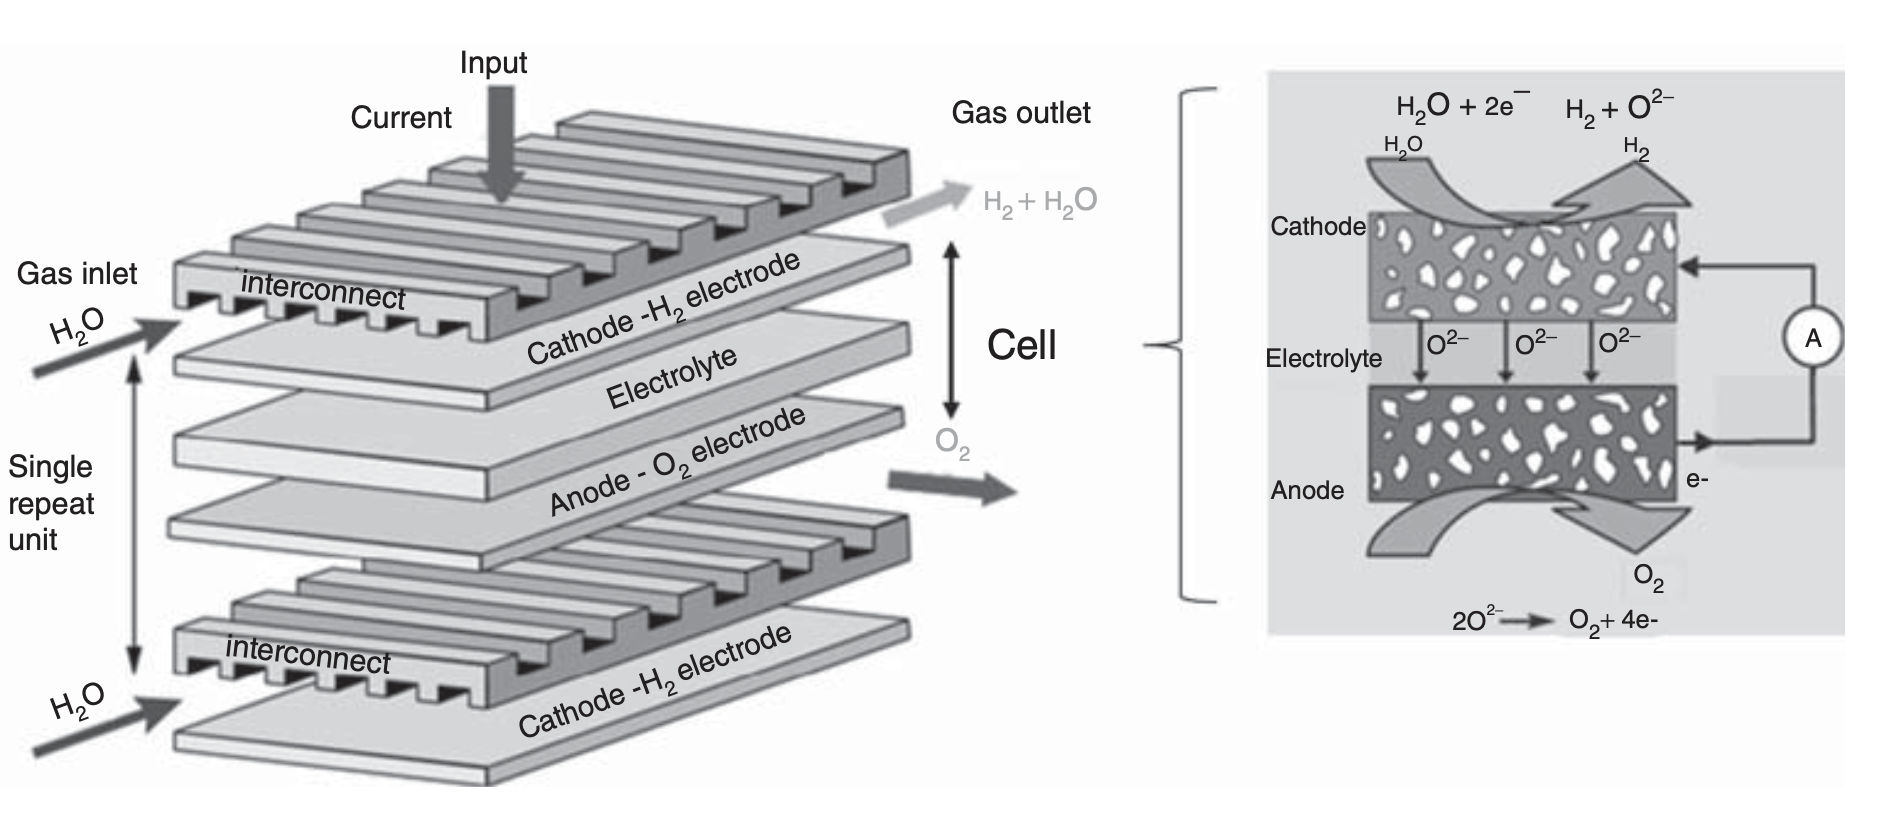
\includegraphics[width=0.4\textwidth]{cf89a71a-2c53-11eb-895f-8c8590753a48.png}
	\caption{The schematic for a single cell of a solid-oxide fuel cell.}
	\label{fig:SE_cell}
\end{figure}
At these temperatures the reaction can proceed faster than at the lower temperatures (\SI{>100}{\celsius}), resulting in a higher electrical efficiency\cite{Schiller2019}.
Overpotential is a major issue with current methods of water electrolysis so overcoming this in systems operating at scale is an important step.

Splitting water in this reaction occurs at two sites; the fuel electrode proceeds via reaction \eqref{eq:SE_fuel_electrode} and the air electrode via \eqref{eq:SE_air_electrdoe}.\cite{Schiller2019}

\begin{align}
	\ce{H2O + 2e- &-> H2 +O^2-}\label{eq:SE_fuel_electrode}\\
	\ce{O^2- &-> 1/2O2 + 2e-}\label{eq:SE_air_electrode}
.\end{align}

From a thermodynamic perspective the enthalpy required to split water is reduced, as the total enthalpy $\Delta_{r}H$ is significantly lowered by removing the need to supply the enthalpy of vaporisation $\Delta_{\text{vap}}H$, approximately \SI{40.65}{\kilo\joule\per\mole}\cite{Lemmon2017}.
SOECs operating a steam electrolysis reaction have the potential to significantly offset electrical load; the method presented in the paper uses solar energy to superheat water in a steam generator; this is pressurised in an accumulator and fed into the SOEC. 

There are several limitations to this research, while it addresses the possibility of superheating water using solar energy, the experimental set-up uses a solar simulator which is obviously an ideal condition, making this not necessarily geographically suitable.
The SOEC used by the team was a laboratory scale device and could not handle steam mass flow exceeding \SI{0.5}{\kilo\gram\per\hour}, making validating this experiment on a large scale difficult; is solar energy suitable for heating water that can feed a large bank of SOECs, as when lost are kept together they are more thermally efficient.


\subsection{Discussion of water-splitting methods}%
\label{sub:discussion_of_water_splitting_methods}

Acidic/alkaline amphoteric \ce{H2O} electrolytic cells operate below \SI{100}{\celsius}\cite{Lei2019}, whereas solid oxide electrolytic cells (SOEC) operate between \SIrange{700}{1000}{\celsius}\cite{Schiller2019}.
This higher temperature results in faster reactions and therefore lower energy consumption per unit volume of \ce{H2}.

The Gibbs free enthalpy for \ce{H2O} electrolysis decreases as temperature increases.
This means at higher temperatures the amount of electrical energy required for the process is further lowered.
A large part of the thermal energy can be provided by solar energy.
The enthalpy of \ce{H2O(g)}, and therefore the energy consumption for \ce{H2O} electrolysis is lower than for \ce{H2O(l)}.
Therefore, \ce{H2O} electrolysis in SOEC is more energy efficient than in acidic/electrolytic cells.

Another disadvantage of the acidic/alkaline electrolytic cell is that it depends on an expensive pt electrode, whereas the SOEC uses abundant \ce{Ni}, \ce{La}, \ce{Sr}, \ce{Co}, \ce{Fe}, \ce{Zr} and \ce{Y}.
An advantage of the acidic/alkaline electrolytic cell is that it is a slight adaptation of an existing process and it is far simpler.
It only consists of one main component, whereas the SOEC consists of five.
This means it is likely to be more reliable and easier to maintain.
Since one of the biggest issues facing the commercial production of \ce{H2} from \ce{H2O} is the energy consumption, with further refinement the SOEC looks to have the most potential.




\section{Conclusion}%
\label{sec:conclusion}
 \ce{H2O} can be obtained more easily than  \ce{CH4}, which requires extraction from natural gas or the decomposition of biomass.
 \ce{H2O} is also inert and therefore far safer than  \ce{CH4} which is flammable.
Additionally,  \ce{H2O} is far easier to transport because it is a liquid above \SI{0}{\celsius}.
\ce{CH4} is a gas with a boiling point of \SI{-161.5}{\celsius}, therefore to transport large quantities it must be stored at very low temperatures as liquified natural gas \cite{lngamerica}.

However, in some locations where  \ce{H2O} is sparse or there is an unreliable electricity supply,  \ce{CH4} is a good solution\cite{SBN2020}.
Therefore, innovation is required for methods using both feedstocks.

The recent developments in water electrolysis and methane decomposition covered by this review are very promising alternatives to the methods currently used commercially.
Each paper recognises the challenges facing the large-scale use of a new method and takes steps to address these issues.
A method using  \ce{CH4} that stands out is radical methane decomposition (RMD), which requires \SI{11}{\percent} of the enthalpy required for traditional steam methane reformation.
A method using  \ce{H2O} that stands out is solid oxide steam electrolysis (SOSE), which uses less energy than traditional electrolysis and can use solar thermal energy to provide a significant portion.

Neither of these techniques are perfect, for example the RMD produces carbon as a waste product which greatly limits the lifespan of the catalyst and SOSE has issues maintaining the steam supply.
However, with further refinement, these cutting-edge techniques have potential to replace the flawed methods currently favoured for the industrial production of  \ce{H2}.


%\bibliography{../Citations/bibtool}
\bibliography{bibtool}
\bibliographystyle{rsc}

\end{multicols}
\end{document}

